\section{19.11.2014 - Porte logiche II}

In questa esperienza studieremo le porte logiche TTL in maniera più approfondita e ne cercheremo di capire le problematiche. Analizzeremo porte tri-state e costruiremo un circuito di multiplexing.

\subsection*{Strumenti e materiali}

\begin{itemize} [noitemsep]
	\item Oscilloscopio Agilent DSO-X 2002A (bandwidth \SI{70}{\mega\hertz}, sample rate \num{2} GSa/s);
	\item Generatore di tensione continua Agilent E3631A (max $\pm \, \SI{25}{\volt}$ o $\pm \, \SI{6}{\volt}$);
	\item Multimetro Agilent 34410A a sei cifre e mezza;
	\item Un integrato 7400, composto di quattro porte logiche TTL NAND; % '00;
	\item Un integrato 74LS05, composto di quattro porte logiche NOT TTL Open Collector;
	\item Un integrato 74LS125, composto di quattro porte logiche buffer TTL 3State;
	\item Basetta a LED;		
	\item Resistenze e capacità di vari valori;
	\item Breadboard e cablaggi vari.
\end{itemize}

\subsection{Tempo di propagazione}

\begin{wrapfigure}[10]{l}{0.5\textwidth}
\centering
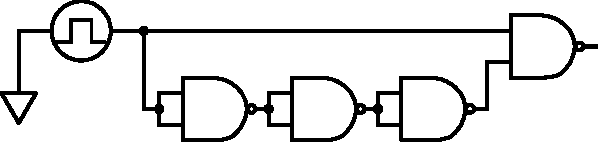
\includegraphics[width=.4\textwidth]{../E10/latex/delay.pdf}
\caption{Schema del circuito utilizzato per misurare il Propagation Delay Time (PDT) di una porta NAND.}
\label{cir10:delay}
\end{wrapfigure}


In questa prima parte dell'esperienza analizzeremo il PDT (Propagation Delay Time) di una porta NAND.
Tale parametro è il ritardo con cui l'uscita commuta rispetto all'istante in cui commuta l'ingresso.
Poichè tale intervallo temporale è di pochi \si{\nano\second}, è stato deciso di collegare in serie 3 porte NOT.
Così facendo il ritardo viene amplificato di 3 volte.
Possiamo ora costruire il circuito riportato in Figura \ref{cir10:delay}.

Come vediamo, se non esistesse il ritardo l'uscita sarebbe sempre ad 1 logico ($\approx 5 \si{\volt}$).
A causa del ritardo, però, quando il segnale in ingresso commuta da 0 ad 1, la serie di porte NOT non riuscità instantaneamente a passare da 1 a 0 e dunque, per un breve intervallo entrambi gli ingressi saranno ad 1 logico il che implica un uscita a 0 logico.
Abbiamo utilizzato in ingresso un'onda quadra ($V_{pp}=\SI{5}{\volt}$, $V_{off}=+\SI{2.5}{\volt}$, $\nu=\SI{100}{\kilo\hertz}$).
Notiamo che la presenza della porta NAND in uscita non da contributo al ritardo totale in quanto essa provoca solo uno shift temporale, non un aumento del delay.
Il valore ch stimeremo dal grafico dovrà dunque essere diviso per 3, in modo da ottenere il tempo di propagazione di una singola porta.

\begin{figure}[htpc]
\centering
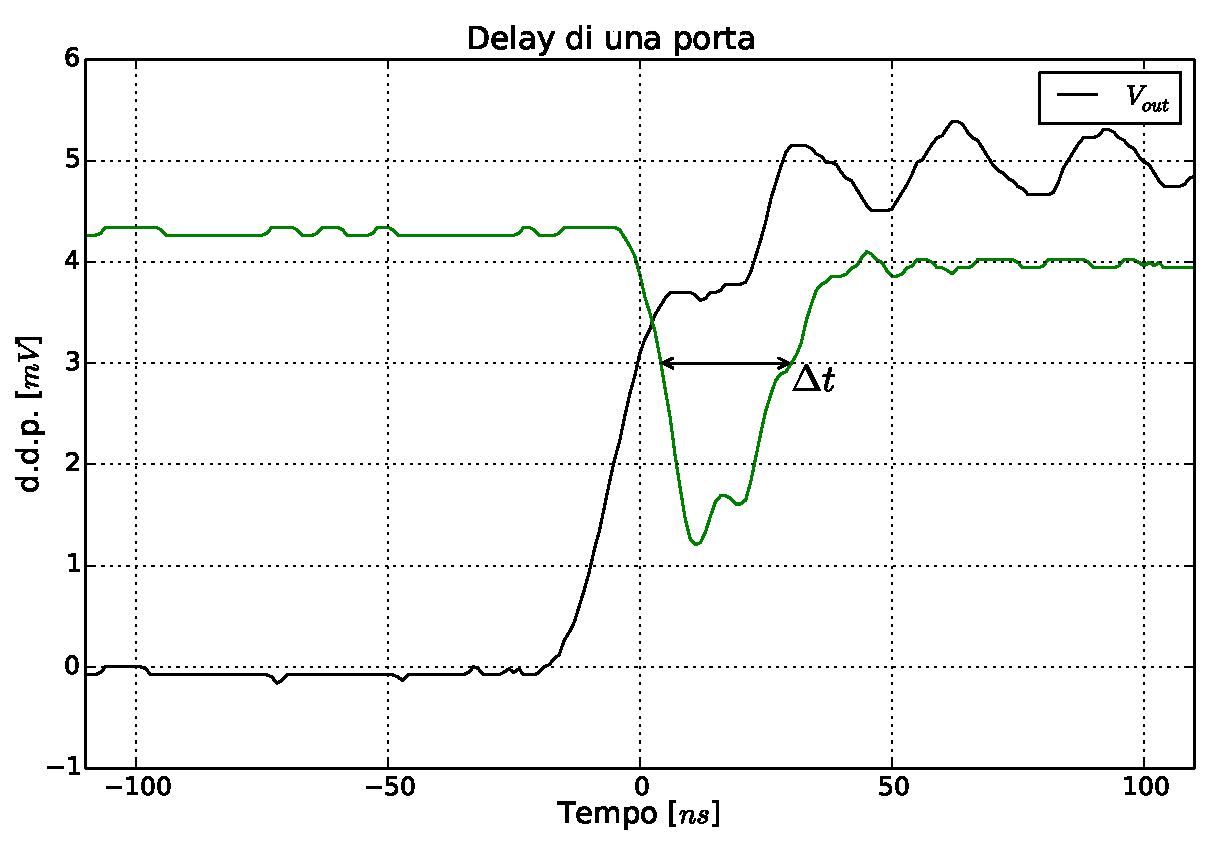
\includegraphics[width=.65\textwidth]{../E10/latex/gdelay.pdf}
\caption{Grafico che mostra la risposta la risposta in uscita del circuito in Figura \ref{cir10:delay} al cambiamento di stato (da 0 a \SI{5}{\V}) dell'onda quadra in ingresso.}
\label{gr10:delay}
\end{figure}

Come vediamo il segnale non è perfettamente un'onda quadra, nè in ingresso nè in uscita.
Ciò è dovuto alle impedenze parassite e alle correnti assorbite dalla porta.
Abbiamo dunque deciso di prendere i valori temporali al 50\% dell'ampiezza massima.
I valori ottenuti sono \SI{26\pm 2}{\nano\second}.
Il valore Per la singola porta è dunque \SI{9\pm 1}{\nano\second}, valore compatibile con i valori riportati sul datasheet.

\subsection{Verifica di una porta NOT TTL Open Collector }

\begin{wrapfigure}[17]{r}{0.3\textwidth}
\centering
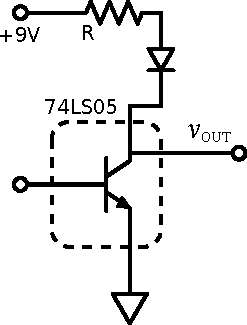
\includegraphics[width=.2\textwidth]{../E10/latex/open_collector.pdf}
\caption{Schema del circuito utilizzato per la verifica di funzionamento di una porta NOT open collector.}
\label{cir10:open_collector}
\end{wrapfigure}

Questa seconda parte dell'esperienza prevede la verifica di una porta NOT TTL Open Collector.
Tali porte sono particolarmente utili quando vogliamo passare tra logiche che lavorano a tensioni diverse.
Infatti, avendo il collettore aperto, possiamo collegare il collettore stesso ad una tensione diversa rispetto a quella con cui è alimentata la porta.
Nel nostro caso, abbiamo utilizzato una porta TTL (0/+5 \si{\volt}) e abbiamo collegato il collettore a +9\si{\volt}.
Per la verifica abbiamo deciso di utilizzare un led luminoso.
Lo schema circuitale è riportato in Figura \ref{cir10:open_collector}.

Considerando una caduta di circa \SI{1.5}{\volt} sul led e una corrente di \SI{5}{\milli\ampere}, e una caduta data dal transistor della porta di circa \SI{0.5}{\volt} possiamo facilmente calcolare, usando la legge di Ohm, la resistenza necessaria.
Il valore scelto alla fine anche per comodità è di \SI{1.5}{\kilo\ohm}.

Ricordiamo che il transistor che compone la nostra porta sarà in saturazione quando la tensione in ingresso è alta, e dunque avremo un'uscita bassa.
Invece, quando all'ingresso avremo uno zero logico, il transistor sarà interdetto e dunque avremo una tensione alta in uscita.


Il circuito è stato verificato infine utilizzando l'oscilloscopio.
I dati sono riportati nel seguente grafico.

\begin{figure}[htpc]
\centering
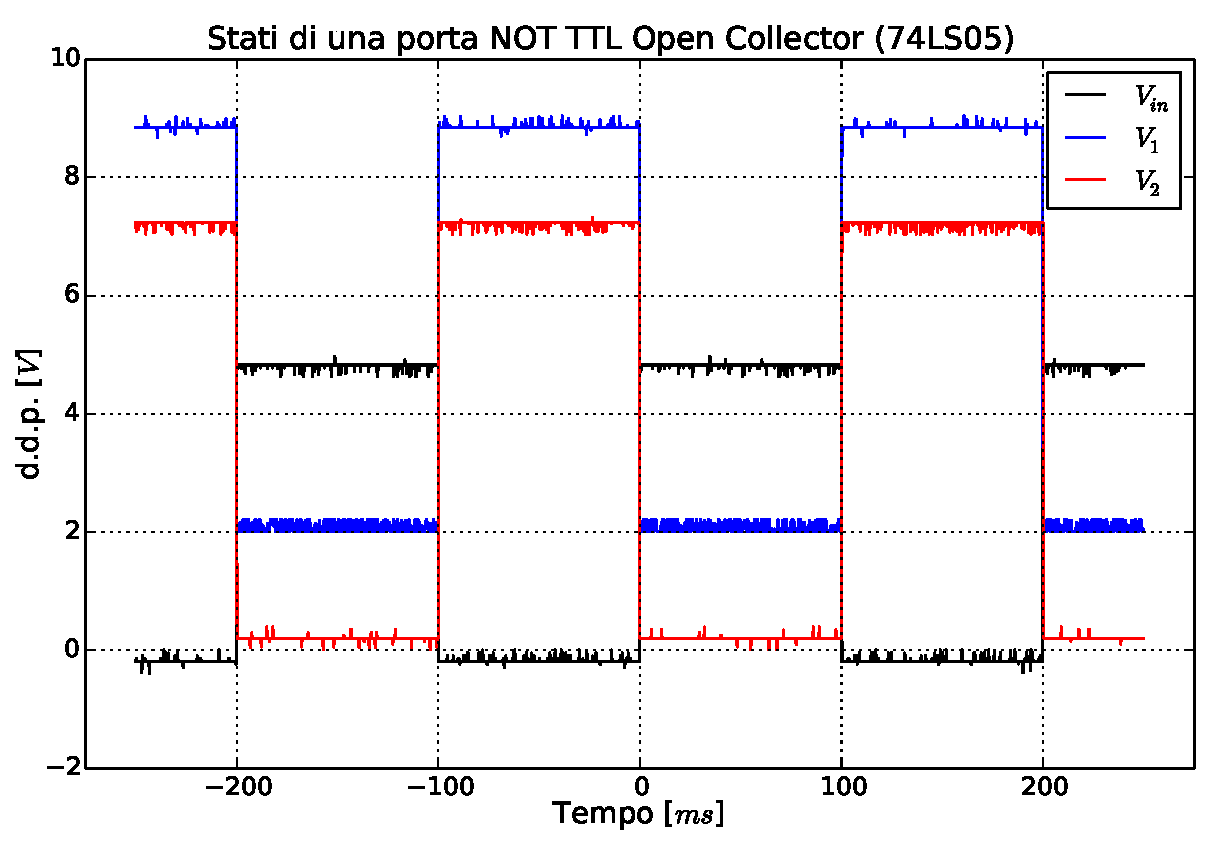
\includegraphics[width=.65\textwidth]{../E10/latex/NOTTTL.pdf}
\caption{Grafico che mostra l'onda in entrata e la risposta del circuito presa in due punti differenti: $V_1$ è stata misurata tra la resistenza $R$ e il diodo, mentre $V_2$ è stata misurata tra il diodo e l'uscita della porta NOT.}
\label{gr10:notttl}
\end{figure}

Come vediamo dal grafico, la tensione di 0 logico è circa \SI{0.4}{\volt}, valore coerente con quello atteso data la caduta della giungione base-emettitore del transistor.
Tuttavia, se preleviamo la tensione in uscita sotto il diodo, abbiamo come tensione alta \SI{7.4}{\V}.
Ciò non è aspettato in quanto dovremmo trovare la stessa tensione di alimentazione (+\SI{9}{\V}).
Abbiamo allora provato a prelevare la tensione sopra il diodo, ottendendo una tensione alta di \SI{9}{\V} ed una bassa di \SI{2}{\V}.
Tale valore, ovviamente, è dovuto al fatto che abbiamo una caduta sia sul diodo ($\approx \SI{1.5}{\V}$) sia sul transistor ($\approx$ \SI{0.5}{\V}).

Abbiamo provato a misurare, utilizzando l'amperometro, la corrente che scorre nel ramo di collettore.
Il risultato ottenuto è che la corrente è dell'ordine dei \si{\micro\ampere}, cosa aspettata  in quanto il transistor è in interdizione.
Non siamo riusciti a capire perchè il diodo provocasse una caduta in tensione di $\approx \SI{1.5}{\volt}$ anche quando attraverso esso non scorreva corrente.

\newpage
\subsection{Verifica di una porta buffer TTL 3State}

\begin{wrapfigure}[14]{l}{0.5\textwidth}
\centering
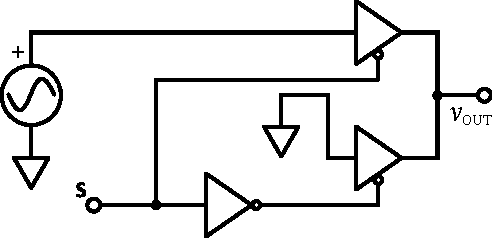
\includegraphics[width=.4\textwidth]{../E10/latex/impedence.pdf}
\caption{Circuito per trasmissione \textit{half duplex} costruito mediante l'utilizzo di porte 3State. Esso permette di condividere lo stesso canale trasmissivo.}
\label{cir10:3state}
\end{wrapfigure}

In questa parte abbiamo realizzato un circuito per trasmissione half-duplex tramite porte 3State.
Il fine di tale operazione è quello di condividere lo stesso canale per la trasmissione dei dati.
Possiamo dunque, semplicemente cambiando il segnale di controllo, decidere quale segnale deve essere trasmesso.
Ciò, come si vedrà nella seguente sezione, è particolarmente utile nel caso in cui si abbiano molti segnali da trasmettere.
Il circuito da noi implementato è quello riportato in figura.
Ricordiamo che le porte 3State da noi utilizzate sono attivate se il controllo è a 0 logico mentre sono ad "alta impedenza" se il controllo è ad 1 logico.
Dunque il circuito da noi costruito permetterà di selezionare uno dei due segnali e, sfruttando lo stato "alta impedenza", evitiamo cortocircuiti tra le uscite.

Il circuito è stato testato utilizzando la schedina a led.


\subsection{Trasmissione di segnali}

In questa parte dell'esperienza ci occuperemo di effettuare la trasmissione di segnali attraverso un circuito logico.
Ovviamente potremmo dedicare ad ogni segnale un filo: dunque, se volessimo trasportare $N$ segnali dovremmo utilizzare $N$ fili.

\begin{wrapfigure}[13]{l}{0.5\textwidth}
\centering
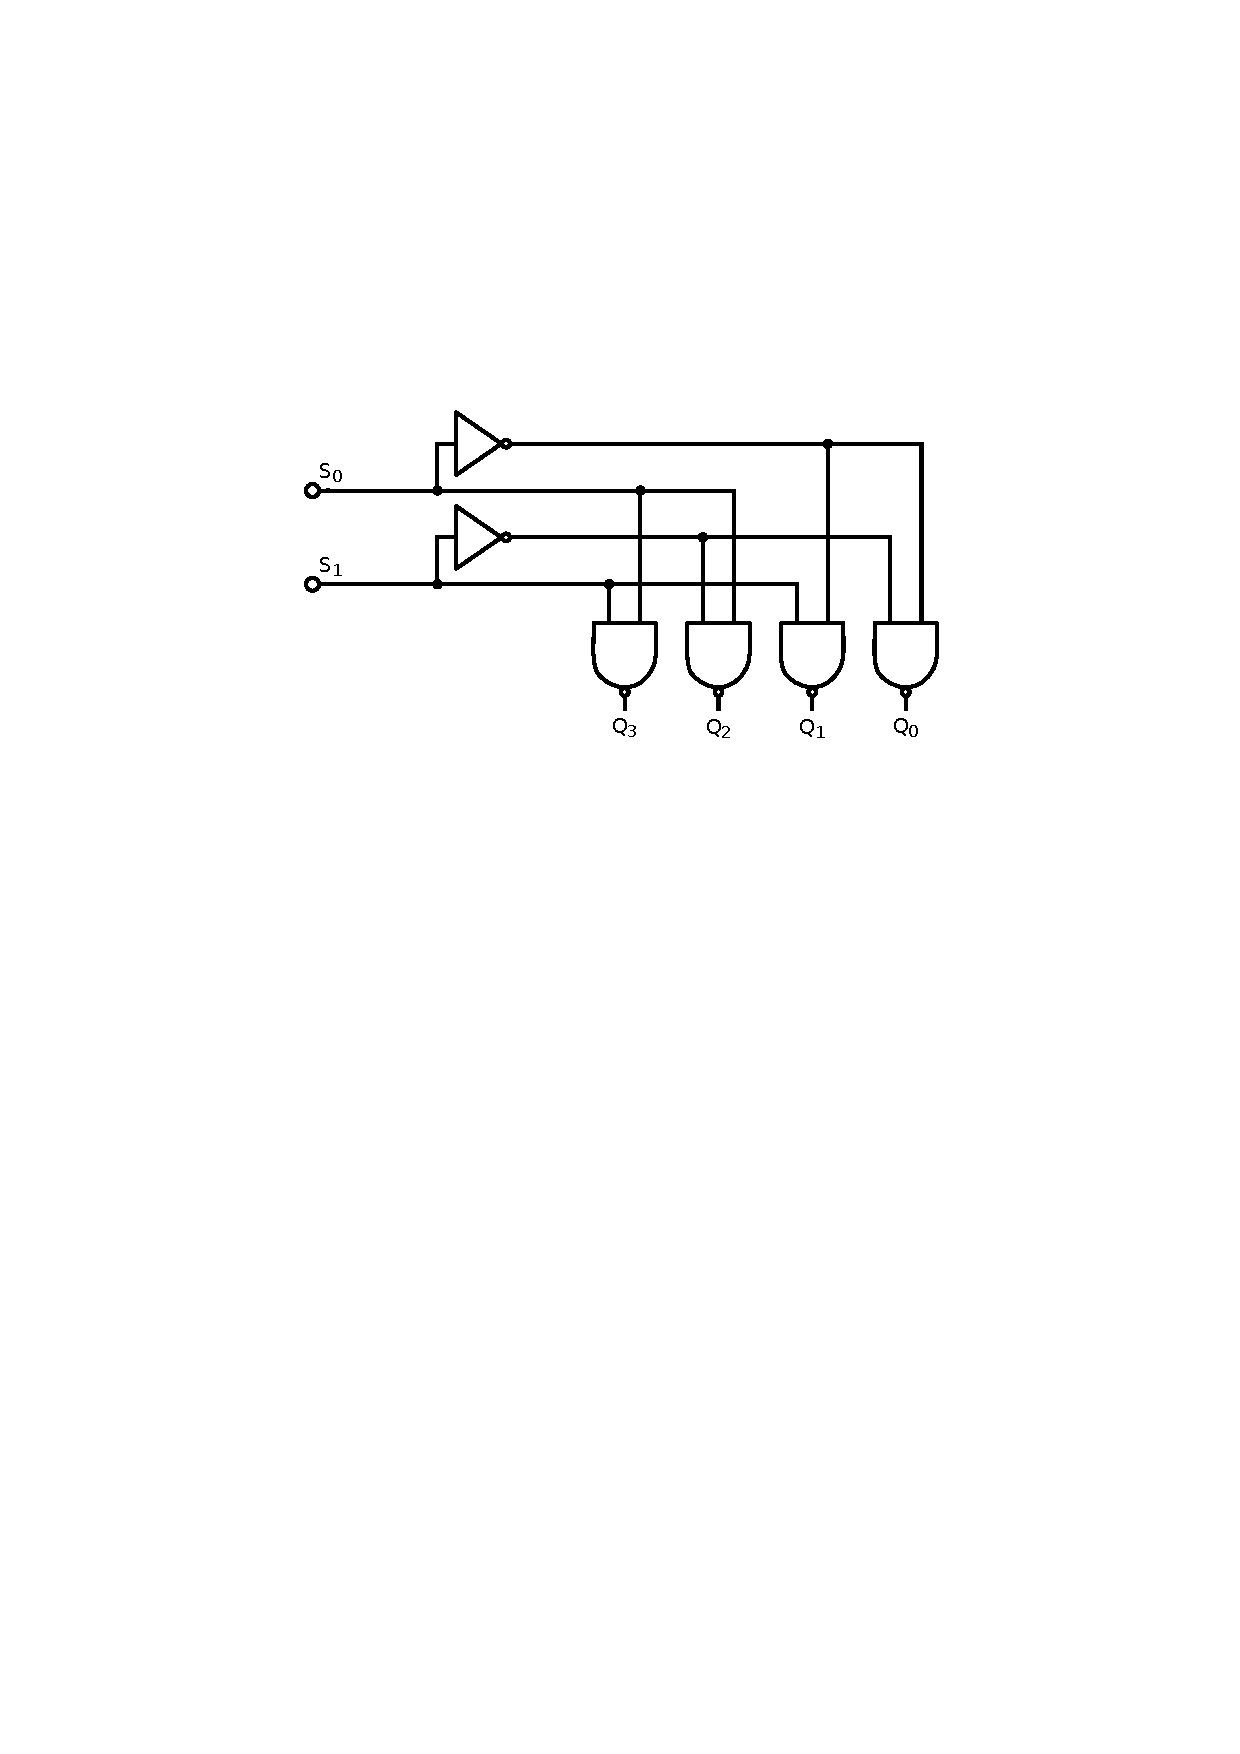
\includegraphics[width=.38\textwidth]{../E10/latex/selector.pdf}
\caption{Schema circuitale della parte dedicata alla selezione del canale in utilizzo per la comunicazione.}
\label{cir10:selector}
\end{wrapfigure}

Un modo più efficiente è segnalare a chi deve ricevere il segnale quale di questi $N$ segnali stia passando su un unico cavo di trasmissione.
Dobbiamo quindi predisporre una circuiteria dedicata al \textit{segnale di selezione} e dovremmo portare tanti cavi quanti siano necessari ad identificare univocamente tutti gli $N$ segnali.

Ad esempio, nel nostro caso abbiamo bisogno di mandare quattro segnali distinti, quindi avremo bisogno di due segnali di selezione (infatti le combinazioni di 1 e 0 logici possibili sono abbastanza per assegnare ad ognuno dei quattro segnali un codice logico di due cifre).
Dunque, insieme al cavo dedicato alla trasmissione dati e a quello di terra (abbiamo bisogno di un riferimento comune per i nostri stati logici), costruiremo un circuito di trasmissione che utilizzerà quattro cavi e avrà bisogno di blocchi per la selezione e blocchi per la trasmissione.

\subsubsection{Selettore}

Per permettere la selezione del segnale abbiamo bisogno di implementare la seguente tabella di verità (con $S_0$ ed $S_1$ i segnali di selezione che passeranno sui due cavi di selezione).

\begin{table}[htpc]
\centering
{\renewcommand{\arraystretch}{1.1}%
\begin{tabular}{|c|c|c|c|c|c|}
\hline
$S_0$ & $S_1$ & $Q_0$ & $Q_1$ & $Q_2$ & $Q_3$ \\
\hline
0 & 0 & 0 & 1 & 1 & 1\\
\hline
0 & 1 & 1 & 0 & 1 & 1\\
\hline
1 & 0 & 1 & 1 & 0 & 1\\
\hline
1 & 1 & 1 & 1 & 1 & 0\\
\hline
\end{tabular}}
\label{tab10:multiplx_selezione}
\end{table}

\begin{wraptable}[9]{c}{.3\textwidth}
\centering
{\renewcommand{\arraystretch}{1}%
\begin{tabular}{|c|c|c|}
\hline
\diaghead{\theadfont lololololo a} {$S_0$}{$S_1$}& 0 & 1\\
\hline
0 & 0 & 1\\
\hline
1 & 1 & 1\\
\hline
\end{tabular}}
\caption{}
\label{tab10:multiplex_selezione_Q}
\end{wraptable}

In questo modo in uscita avremo come 0 solo la $Q_i$ relativa al segnale selezionato con i due segnali di selezione.

Per far ciò, possiamo dividere il problema come se ogni $Q_i$ abbia una mappa di Karnaugh associata come in Tabella \ref{tab10:multiplex_selezione_Q}\footnote{Lo svolgiamo per $Q_0$ ma gli altri tre casi sono analoghi}.

Otteniamo dunque, considerando per ogni mappa lo 0 come stato logico che ci interessa
$$Q_0 = \overline S_0 \overline S_1 \quad Q_1 = S_0 \overline S_1 \quad Q_0 = \overline S_0 S_1 \quad Q_3 = S_0  S_1$$

E' dunque facile vedere che una implementazione di questo sistema è il circuito logico in Figura \ref{cir10:selector}.

\newpage
\subsubsection{Multiplexing}

\begin{wrapfigure}[14]{r}{0.45\textwidth}
\centering
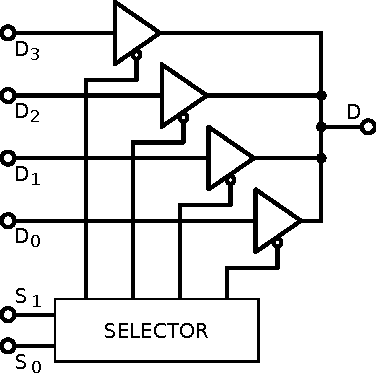
\includegraphics[width=.25\textwidth]{../E10/latex/mult.pdf}
\caption{Schema circuitale della parte dedicata al multiplexing dei segnali.}
\label{cir10:mult}
\end{wrapfigure}

Dati i segnali $Q_i$ del circuito di selezione, ora dobbiamo implementare un circuito che passi al cavo di trasmissione solo il segnale che ci interessa.
Possiamo dunque utilizzare delle porte tri-state con ingresso di attivazione negato; infatti, collegando a questo ingresso uno dei segnali $Q_i$, faremo passare il segnale $D_i$ (collegato all'altro ingresso della tri-state) se e solo se $Q_i=0$.

Un altro vantaggio di utilizzare le tri-state è quello di avere un'alta impedenza quando $Q_i$ viene posto ad 1 logico (e dunque il segnale selezionato è un altro), evitando cortocircuiti alle uscite delle tri-state (sono tutte collegate al cavo di trasmissione).

Il circuito di multiplexing è riportato in Figura \ref{cir10:mult}.

\subsubsection{De-multiplexing}

\begin{wrapfigure}[14]{r}{0.45\textwidth}
\centering
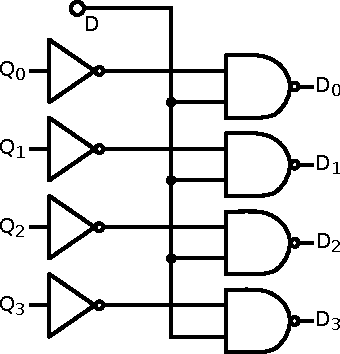
\includegraphics[width=.25\textwidth]{../E10/latex/demult.pdf}
\caption{Schema circuitale della parte dedicata al de-multiplexing dei segnali.}
\label{cir10:demult}
\end{wrapfigure}

Portando i segnali $S_0$ ed $S_1$ di chi invia il segnale ad un selettore (uguale al precedente), il ricevente può costruire un circuito che passi in uscita il dato inviato.

Per far ciò, dobbiamo innanzitutto negare i segnali $Q_i$ (si veda tabella del selettore) per poi inviarli separatamente ad una porta AND: considerandola come un interruttore, e collegando le altre entrate al cavo di trasmissione, avremo in uscita dedicata solo il dato richiesto, e sugli altri lo 0 logico.
Il circuito di de-multiplexing è in Figura \ref{cir10:demult}.


\subsection*{Conclusioni}

In questa esperienza siamo riusciti a valutare il ritardo del segnale in uscita da una porta ed il funzionamento di una porta NOT TTL in configurazione Open Collector e di una TTL Tri-State.

Abbiamo infine verficato il funzionamento di un sistema che utilizza il multiplexing per trasmettere vari segnali-dati. È così possibile ridurre il numero di cavi (e dunque il costo in denaro e spazio) per trasmettere N-segnali.
